\hypertarget{day-8---ux6784ux5efaux524dux7aef}{%
\subsection{Day 8 - 构建前端}\label{day-8---ux6784ux5efaux524dux7aef}}

虽然我们跑通了一个最简单的 MVC,但是页面效果肯定不会让人满意。

对于复杂的 HTML 前端页面来说,我们需要一套基础的 CSS
框架来完成页面布局和基本样式。另外,jQuery 作为操作 DOM 的 JavaScript
库也必不可少。

从零开始写 CSS 不如直接从一个已有的功能完善的 CSS 框架开始。有很多 CSS
框架可供选择。我们这次选择 \href{http://getuikit.com/}{uikit} 这个强大的
CSS 框架。它具备完善的响应式布局,漂亮的 UI,以及丰富的 HTML
组件,让我们能轻松设计出美观而简洁的页面。

可以从 \href{http://getuikit.com/}{uikit 首页}下载打包的资源文件。

所有的静态资源文件我们统一放到\texttt{www/static}目录下,并按照类别归类:

\begin{pythoncode}
static/
+- css/
|  +- addons/
|  |  +- uikit.addons.min.css
|  |  +- uikit.almost-flat.addons.min.css
|  |  +- uikit.gradient.addons.min.css
|  +- awesome.css
|  +- uikit.almost-flat.addons.min.css
|  +- uikit.gradient.addons.min.css
|  +- uikit.min.css
+- fonts/
|  +- fontawesome-webfont.eot
|  +- fontawesome-webfont.ttf
|  +- fontawesome-webfont.woff
|  +- FontAwesome.otf
+- js/
   +- awesome.js
   +- html5.js
   +- jquery.min.js
   +- uikit.min.js
\end{pythoncode}

由于前端页面肯定不止首页一个页面,每个页面都有相同的页眉和页脚。如果每个页面都是独立的
HTML
模板,那么我们在修改页眉和页脚的时候,就需要把每个模板都改一遍,这显然是没有效率的。

常见的模板引擎已经考虑到了页面上重复的 HTML 部分的复用问题。有的模板通过
include 把页面拆成三部分:

\begin{pythoncode}
<html>
    <% include file="inc_header.html" %>
    <% include file="index_body.html" %>
    <% include file="inc_footer.html" %>
</html>
\end{pythoncode}

这样,相同的部分\texttt{inc\_header.html}和\texttt{inc\_footer.html}就可以共享。

但是 include 方法不利于页面整体结构的维护。jinjia2 的模板还有另一种
``继承'' 方式,实现模板的复用更简单。

``继承'' 模板的方式是通过编写一个 ``父模板'',在父模板中定义一些可替换的
block(块)。然后,编写多个
``子模板'',每个子模板都可以只替换父模板定义的
block。比如,定义一个最简单的父模板:

\begin{pythoncode}
<html>
    <head>
        <title> 这里定义了一个名为title的block </title>
    </head>
    <body>
         这里定义了一个名为content的block 
    </body>
</html>
\end{pythoncode}

对于子模板\texttt{a.html},只需要把父模板的\texttt{title}和\texttt{content}替换掉:

\begin{pythoncode}


 A 


    <h1>Chapter A</h1>
    <p>blablabla...</p>

\end{pythoncode}

对于子模板\texttt{b.html},如法炮制:

\begin{pythoncode}


 B 


    <h1>Chapter B</h1>
    <ul>
       <li>list 1</li>
       <li>list 2</li>
    </ul>

\end{pythoncode}

这样,一旦定义好父模板的整体布局和 CSS 样式,编写子模板就会非常容易。

让我们通过 uikit 这个 CSS
框架来完成父模板\texttt{\_\_base\_\_.html}的编写:

\begin{pythoncode}
<!DOCTYPE html>
<html>
<head>
    <meta charset="utf-8" />
    
    <title> ?  - Awesome Python Webapp</title>
    <link rel="stylesheet" href="/static/css/uikit.min.css">
    <link rel="stylesheet" href="/static/css/uikit.gradient.min.css">
    <link rel="stylesheet" href="/static/css/awesome.css" />
    <script src="/static/js/jquery.min.js"></script>
    <script src="/static/js/md5.js"></script>
    <script src="/static/js/uikit.min.js"></script>
    <script src="/static/js/awesome.js"></script>
    
</head>
<body>
    <nav class="uk-navbar uk-navbar-attached uk-margin-bottom">
        <div class="uk-container uk-container-center">
            <a href="/" class="uk-navbar-brand">Awesome</a>
            <ul class="uk-navbar-nav">
                <li data-url="blogs"><a href="/"><i class="uk-icon-home"></i> 日志</a></li>
                <li><a target="_blank" href="#"><i class="uk-icon-book"></i> 教程</a></li>
                <li><a target="_blank" href="#"><i class="uk-icon-code"></i> 源码</a></li>
            </ul>
            <div class="uk-navbar-flip">
                <ul class="uk-navbar-nav">
                
                    <li class="uk-parent" data-uk-dropdown>
                        <a href="#0"><i class="uk-icon-user"></i> {{ user.name }}</a>
                        <div class="uk-dropdown uk-dropdown-navbar">
                            <ul class="uk-nav uk-nav-navbar">
                                <li><a href="/signout"><i class="uk-icon-sign-out"></i> 登出</a></li>
                            </ul>
                        </div>
                    </li>
                
                    <li><a href="/signin"><i class="uk-icon-sign-in"></i> 登陆</a></li>
                    <li><a href="/register"><i class="uk-icon-edit"></i> 注册</a></li>
                
                </ul>
            </div>
        </div>
    </nav>

    <div class="uk-container uk-container-center">
        <div class="uk-grid">
            
            
            
            
        </div>
    </div>

    <div class="uk-margin-large-top" style="background-color:#eee; border-top:1px solid #ccc;">
        <div class="uk-container uk-container-center uk-text-center">
            <div class="uk-panel uk-margin-top uk-margin-bottom">
                <p>
                    <a target="_blank" href="#" class="uk-icon-button uk-icon-weibo"></a>
                    <a target="_blank" href="#" class="uk-icon-button uk-icon-github"></a>
                    <a target="_blank" href="#" class="uk-icon-button uk-icon-linkedin-square"></a>
                    <a target="_blank" href="#" class="uk-icon-button uk-icon-twitter"></a>
                </p>
                <p>Powered by <a href="#">Awesome Python Webapp</a>. Copyright © 2014. [<a href="/manage/" target="_blank">Manage</a>]</p>
                <p><a href="http://www.liaoxuefeng.com/" target="_blank">www.liaoxuefeng.com</a>. All rights reserved.</p>
                <a target="_blank" href="#"><i class="uk-icon-html5" style="font-size:64px; color: #444;"></i></a>
            </div>
        </div>
    </div>
</body>
</html>
\end{pythoncode}

\texttt{\_\_base\_\_.html}定义的几个 block 作用如下:

用于子页面定义一些 meta,例如 rss feed:

\begin{pythoncode}
 ... 
\end{pythoncode}

覆盖页面的标题:

\begin{pythoncode}
 ... 
\end{pythoncode}

子页面可以在\texttt{\textless{}head\textgreater{}}标签关闭前插入
JavaScript 代码:

\begin{pythoncode}
 ... 
\end{pythoncode}

子页面的 content 布局和内容:

\begin{pythoncode}

    ...

\end{pythoncode}

我们把首页改造一下,从\texttt{\_\_base\_\_.html}继承一个\texttt{blogs.html}:

\begin{pythoncode}


日志



    <div class="uk-width-medium-3-4">
        
            <article class="uk-article">
                <h2><a href="/blog/{{ blog.id }}">{{ blog.name }}</a></h2>
                <p class="uk-article-meta">发表于{{ blog.created_at}}</p>
                <p>{{ blog.summary }}</p>
                <p><a href="/blog/{{ blog.id }}">继续阅读 <i class="uk-icon-angle-double-right"></i></a></p>
            </article>
            <hr class="uk-article-divider">
        
    </div>

    <div class="uk-width-medium-1-4">
        <div class="uk-panel uk-panel-header">
            <h3 class="uk-panel-title">友情链接</h3>
            <ul class="uk-list uk-list-line">
                <li><i class="uk-icon-thumbs-o-up"></i> <a target="_blank" href="#">编程</a></li>
                <li><i class="uk-icon-thumbs-o-up"></i> <a target="_blank" href="#">读书</a></li>
                <li><i class="uk-icon-thumbs-o-up"></i> <a target="_blank" href="#">Python教程</a></li>
                <li><i class="uk-icon-thumbs-o-up"></i> <a target="_blank" href="#">Git教程</a></li>
            </ul>
        </div>
    </div>


\end{pythoncode}

相应地,首页 URL 的处理函数更新如下:

\begin{pythoncode}
@get('/')
def index(request):
    summary = 'Lorem ipsum dolor sit amet, consectetur adipisicing elit, sed do eiusmod tempor incididunt ut labore et dolore magna aliqua.'
    blogs = [
        Blog(id='1', name='Test Blog', summary=summary, created_at=time.time()-120),
        Blog(id='2', name='Something New', summary=summary, created_at=time.time()-3600),
        Blog(id='3', name='Learn Swift', summary=summary, created_at=time.time()-7200)
    ]
    return {
        '__template__': 'blogs.html',
        'blogs': blogs
    }
\end{pythoncode}

Blog 的创建日期显示的是一个浮点数,因为它是由这段模板渲染出来的:

\begin{pythoncode}
<p class="uk-article-meta">发表于{{ blog.created_at }}</p>
\end{pythoncode}

解决方法是通过 jinja2 的
filter(过滤器),把一个浮点数转换成日期字符串。我们来编写一个\texttt{datetime}的
filter,在模板里用法如下:

\begin{pythoncode}
<p class="uk-article-meta">发表于{{ blog.created_at|datetime }}</p>
\end{pythoncode}

filter 需要在初始化 jinja2 时设置。相关代码如下:

\begin{pythoncode}
def datetime_filter(t):
    delta = int(time.time() - t)
    if delta < 60:
        return '1分钟前'
    if delta < 3600:
        return '%s分钟前' % (delta // 60)
    if delta < 86400:
        return '%s小时前' % (delta // 3600)
    if delta < 604800:
        return '%s天前' % (delta // 86400)
    dt = datetime.fromtimestamp(t)
    return '%s年%s月%s日' % (dt.year, dt.month, dt.day)

...
init_jinja2(app, filters=dict(datetime=datetime_filter))
...
\end{pythoncode}

现在,完善的首页显示如下:

 
 \begin{figure}[htp]
	\centering
	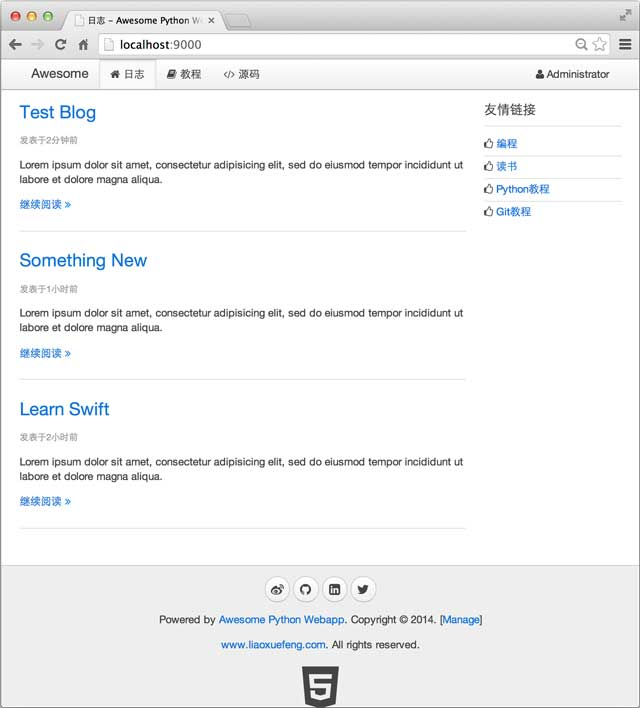
\includegraphics[width=0.6\linewidth]{fig/955626563299584.png}
\end{figure}


\hypertarget{ux53c2ux8003ux6e90ux7801}{%
\subsubsection{参考源码}\label{ux53c2ux8003ux6e90ux7801}}

\href{https://github.com/michaelliao/awesome-python3-webapp/tree/day-08}{day-08}

